%  LaTeX support: latex@mdpi.com
\documentclass[universe,article,submit,oneauthor]{Definitions/mdpi}

\newcommand{\code}{\texttt}
\newcommand{\axionbloch}{\code{axionbloch}}
\newcommand{\python}{\code{Python}}
\newcommand{\scipy}{\code{SciPy}}
\newcommand{\numpy}{\code{NumPy}}
\newcommand{\runtests}{\code{runtests}}
\newcommand{\pytest}{\code{pytest}}
\newcommand{\hdfpy}{\code{h5py}}
\newcommand{\ipython}{\code{IPython}}
\newcommand{\jupyter}{\code{Jupyter}}

\usepackage{graphicx}% Include figure files
% \graphicspath{{../figures/}}

\usepackage{bm}% bold math

%\usepackage[showframe,%Uncomment any one of the following lines to test 
%%scale=0.7, marginratio={1:1, 2:3}, ignoreall,% default settings
%%text={7in,10in},centering,
%%margin=1.5in,
%%total={6.5in,8.75in}, top=1.2in, left=0.9in, includefoot,
%%height=10in,a5paper,hmargin={3cm,0.8in},
%]{geometry}

% %%%%%%%%%%%%%%%%%%%%%%%%%%%%%%%%%%%%%%%%%%%%%%%%%%%%%%%%%%%%%%%%%%%%%%%%%%%%%%%%%%%%%%%%%%%%
 % For professional tables
\usepackage{dcolumn}% Align table columns on decimal point
\usepackage{booktabs} % if you're using \toprule, \midrule, \bottomrule
\usepackage{tabularx}
\usepackage{multirow}
\usepackage{array}
\renewcommand{\arraystretch}{1.5}
% \usepackage{threeparttable}
% %%%%%%%%%%%%%%%%%%%%%%%%%%%%%%%%%%%%%%%%%%%%%%%%%%%%%%%%%%%%%%%%%%%%%%%%%%%%%%%%%%%%%%%%%%%%

% %%%%%%%%%%%%%%%%%%%%%%%%%%%%%%%%%%%%%%%%%%%%%%%%%%%%%%%%%%%%%%%%%%%%%%%%%%%%%%%%%%%%%%%%%%%%
% for chemical forumals
\usepackage{chemformula}
% %%%%%%%%%%%%%%%%%%%%%%%%%%%%%%%%%%%%%%%%%%%%%%%%%%%%%%%%%%%%%%%%%%%%%%%%%%%%%%%%%%%%%%%%%%%%


\usepackage{gensymb} % for degree ° symbol
% \usepackage{float}
%\usepackage{floatrow}
% \usepackage{dblfloatfix}
\usepackage{placeins}
\newenvironment{paperwidefigure}
  {\begin{figurewide}}
  {\end{figurewide}}
\newenvironment{paperwidetable}
  {\begin{table}}
  {\end{table}}
\AtBeginDocument{%
  \crefname{equation}{Equation}{Equations}%
  \Crefname{equation}{Equation}{Equations}%
  \crefname{figurewide}{Figure}{Figures}%
  \Crefname{figurewide}{Figure}{Figures}%
  \crefalias{figurewide}{figure}%
}

% %%%%%%%%%%%%%%%%%%%%%%%%%%%%%%%%%%%%%%%%%%%%%%%%%%%%%%%%%%%%%%%%%%%%%%%%%%%%%%%%%%%%%%%%%%%%
% SI unit
\usepackage{siunitx}
\DeclareSIUnit\torr{torr}
\DeclareSIUnit\ppm{ppm}
\DeclareSIUnit\ppb{ppb}
\DeclareSIUnit\bar{bar}
\DeclareSIUnit\gauss{G}
\DeclareSIUnit\neV{\nano\electronvolt}
\DeclareSIUnit\peV{\pico\electronvolt}
\DeclareSIUnit\kms{km/s}
\sisetup{print-unity-mantissa=false}  % To display only the exponent (i.e., 10⁻¹¹) 
\sisetup{separate-uncertainty = false} % use parenthesis style for uncertainty
% \sisetup{uncertainty-mode = separate} % use +/- style for uncertainty
\sisetup{uncertainty-mode = compact-marker} % turn this on to use style like 123.45(1.20)
% otherwise we  turn this on to use style like 123.45(120)
% %%%%%%%%%%%%%%%%%%%%%%%%%%%%%%%%%%%%%%%%%%%%%%%%%%%%%%%%%%%%%%%%%%%%%%%%%%%%%%%%%%%%%%%%%%%%

\usepackage[normalem]{ulem}
\usepackage{changes}



\usepackage{xcolor}
\newcommand{\JW}[2][cyan]{\textcolor{#1}{Julian: #2}}
\newcommand{\OM}[2][purple]{\textcolor{#1}{Olympia: #2}}
\newcommand{\HB}[2][orange]{\textcolor{#1}{Hendrik: #2}}
\newcommand{\YZ}[2][brown]{\textcolor{#1}{Yuzhe: #2}}
\newcommand{\kp}[2][red]{\textcolor{#1}{* #2}}
\newcommand{\new}[2][red]{\textcolor{#1}{#2}}
\newcommand{\NLF}[2][teal]{\textcolor{#1}{Nate: #2}}
\newcommand{\YG}[2][magenta]{\textcolor{#1}{Younggeun: #2}}
\newcommand{\DB}[2][blue]{\textcolor{#1}{Dima: #2}}


% ----------------------------------------
\firstpage{1}
\makeatletter
\setcounter{page}{\@firstpage}
\makeatother
\pubvolume{1}
\issuenum{1}
\articlenumber{0}
\pubyear{2026}
\copyrightyear{2026}
\datereceived{}
\daterevised{}
\dateaccepted{}
\datepublished{}
\Title{\axionbloch{}: an Open-Source Python Package for Simulating Axion-Induced Spin Dynamics}
\newcommand{\orcidauthorA}{0009-0006-6082-9066}
\Author{Yuzhe Zhang $^{1,2,3}$\orcidA{}}
\AuthorNames{Yuzhe Zhang}
\address{$^{1}$ \quad Johannes Gutenberg-Universit{\"a}t Mainz, 55099 Mainz, Germany\\
$^{2}$ \quad Helmholtz Institute Mainz, 55128 Mainz, Germany\\
$^{3}$ \quad GSI Helmholtzzentrum f{\"u}r Schwerionenforschung GmbH, 64291 Darmstadt, Germany}
\corres{Correspondence: yuhzhang@uni-mainz.de}
\abstract{
The interaction of ultralight bosonic dark matter with spins can be interpreted as a pseudomagnetic field acting on normal matter.
Such interactions can be modeled as usual magnetic interactions using spin-evolution (Bloch) equations.
\axionbloch{}, an open-source Python package for simulating spin dynamics induced by both usual and exotic interactions, is presented. 
The numerical simulations serve as a tool for deriving axion signal signatures, which are crucial for designing experimental searches and data analysis. 
Simulations are calibrated against theoretical expectations, ensuring the accuracy of the simulated signals. 
\axionbloch{} is available at \url{https://github.com/Yuzhe98/AxionBloch}, allowing researchers to simulate pseudomagnetic signals under specific configurations of the axion models and experimental setups. 
The package is documented at \url{http://axionbloch.readthedocs.io/} and includes example scripts for application. 
}
\keyword{axion dark matter; nuclear magnetic resonance; Bloch equations; spin dynamics; Python package}

\begin{document}

\maketitle

\section{Introduction}

The axion was originally proposed to resolve the strong $CP$ problem in quantum chromodynamics\,\cite{PecceiQuinn1977_ConstraintsCP_PRD,Weinberg1978_NewLightBoson,PecceiQuinn1977_CPConservation_PRL,Wilczek1978_ProblemStrongPAndT}. 
Here $C$ denotes charge conjugation and $P$ denotes parity. 
Later, more general axionlike particles (ALPs) were proposed in various extensions of the Standard Model associated with spontaneously broken global symmetries\,\cite{svrcek2006axions,Kim1987_LightPseudoscalars,JaeckelRingwald2010_ALPReview,Arvanitaki2010_StringAxiverse}. 
Concerning the cosmological implications, axions and ALPs are also well-motivated dark matter candidates\,\cite{Preskill1983_invisible_axion,Abbott1983_CosmologicalBoundAxion,Dine1983_not_so_harmless_axion,Marsh2016_AxionCosmology}.
In this paper, axions and ALPs are referred to as ``axions'' for simplicity. 

Axions may possess couplings to ordinary Standard Model particles\,\cite{Graham2013_Newobservables}, including photons, gluons, and fermions. 
Crucially, axion field gradients ($\boldsymbol{\nabla}a$) may couple to fermionic spins through a pseudoscalar interaction. 
The Hamiltonian for this axion--fermion interaction is written as
\begin{equation}
    \mathcal{H}_{\mathrm{int}} = c g_\mathrm{aNN} \boldsymbol{\nabla}a \cdot \boldsymbol{S}\,,
\end{equation}
where $g_\mathrm{aNN}$ is the axion--fermion coupling strength, $c$ is the speed of light, and $\boldsymbol{S}$ denotes the physical spin operator, $\boldsymbol{S}=\hbar\boldsymbol{\sigma}/2$, with $\boldsymbol{\sigma}$ the vector of Pauli matrices. 
The axion field gradient can be regarded as a pseudomagnetic field that mimics the behavior of a real magnetic field, where the Hamiltonian can be written as
\begin{equation}
    \mathcal{H} = -\gamma \boldsymbol{B} \cdot \boldsymbol{S} \,,
\end{equation} 
where $\gamma$ is the gyromagnetic ratio of the spin, and $\boldsymbol{B}$ is the magnetic field. 
Comparing the two Hamiltonians shows that the gradient of the axion field acts effectively as a magnetic field. 
Therefore, the concept of an axion-induced pseudomagnetic field is introduced to represent this effective magnetic field, which is defined as
\begin{equation}
    \boldsymbol{B}_a = -\frac{c g_\mathrm{aNN}}{\gamma}\boldsymbol{\nabla}a\,.
\end{equation}
The precise form of the pseudomagnetic field depends on the axion model.

The pseudomagnetic field induces spin dynamics, providing a pathway for detection in precision measurement experiments such as nuclear magnetic resonance (NMR) and comagnetometer-based searches\,\cite{ouellet2019first, du2018search, ALPHA2023,aja2022canfranc,CAPP2024,brouwer2022projected,alesini2023future,ZhongL2018results,garcia2024searchaxiondarkmatter,Quiskamp2024_ORGAN,rettaroli2024search,Gramolin2021_Ferromagnetic,gavilan2024searching,bloch2105nasduck,abel2023_HgDM,karanth2023first,LeeJunyi2023_NeutronSpin,capozzi2023new, CASPErProposal2014, kimball2018overview, wang2018application, aybas2021_SolidStateNMR, CASPEr_ZULF_2019,Walter2025_CASPErG}. 
There have been dedicated studies of the axion-induced spin dynamics\,\cite{Aybas_2021_Quantum_sensitivity, Dror2023_SensitivityAxion, Yuzhe2023_FrequencyScanning}, providing axion signal signatures and experimental sensitivity to axion fields. 
However, to our knowledge, there have not been studies taking advantage of numerical methods to verify the derived axion signal signatures. 
On the other hand, as more axion models and experiments are being proposed, such as cosmic axion background\,\cite{Dror2021_CosmicAxionBackground,Nitta2023_ADMX_CosmicAxionBackground}, fine-grained axion\,\cite{OHare2025_Finegrained}, and quadratically coupled axion\,\cite{GanXucheng2026_quadraticPTA, huang2026earthmatterenhancedaxion}, a tool is needed to systematically simulate the axion-induced spin dynamics under various physical conditions and axion field configurations.

In this work, \axionbloch{}, an open-source package designed to simulate spin dynamics induced by axion fields, is introduced. 
The interface is implemented in Python, a programming language known for its simplicity and readability, while the underlying numerical integration is implemented in C++ for efficiency. 
The package provides a flexible framework for modeling axion fields and experimental configurations. 
By numerically solving spin-evolution equations, \axionbloch{} enables the prediction and analysis of experimentally observable signals.

\section{Capabilities}
\label{sec:capabilities}

In this section, the main components of \axionbloch{} are described. The section starts with the units, physical quantities, and constants (\cref{sec:units_quantities_constants}). Then, it continues with the physics and the algorithm for the numerical simulation (\cref{sec:algorithm}), after which the calibration for the simulation follows (\cref{sec:calibration}). In the end, an example simulation of axion-induced signals is provided (\cref{sec:simulation}). 


\subsection{Units, physical quantities, and constants}
\label{sec:units_quantities_constants}

The package takes advantage of \texttt{astropy}\footnote{\url{https://astropy.org/}}\,\cite{Astropy2013} to deal with units and physical quantities. 
Using \texttt{astropy.units}, physical quantities are created by attaching units to Python scalars or \texttt{NumPy}\footnote{\url{https://numpy.org/}}\,\cite{Harris2020_NumPy} arrays. 
Quantities can be converted between dimensionally equivalent units using the \texttt{to()} method.
In \texttt{astropy}, unit definitions are included in both the International System of Units (SI) and the Centimeter-Gram-Second (CGS) systems. 
Values in SI or CGS units can be found in the quantity's properties \texttt{.si} and \texttt{.cgs}.
A code example can be found in \cref{code:quantities}. 

In \texttt{axionbloch.constants}, a few commonly-used constants in axion and NMR research, such as gyromagnetic ratios, are defined.
The constants are instances of \texttt{astropy.units.Quantity}; therefore, all operations on physical quantities are supported for the constants. 

\begin{figure}
\center
\fbox{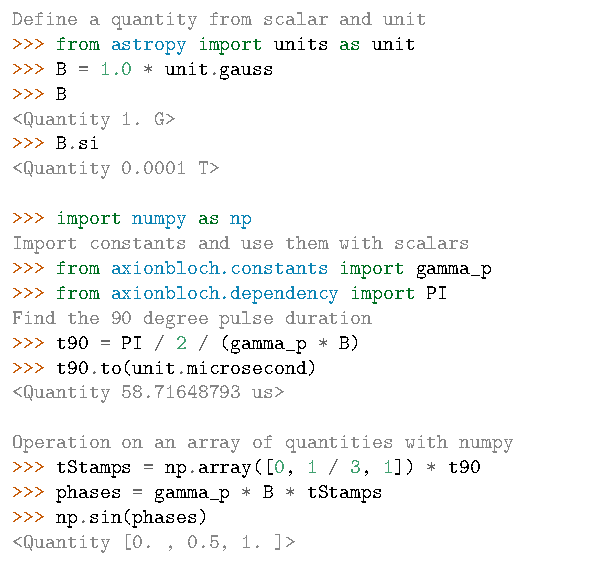
\includegraphics[width=0.45\textwidth,clip]{figures/code_quantities.pdf}}
% \vspace{0.1in}
\caption{Examples of operations on physical quantities using \texttt{astropy.units} and \texttt{axionbloch.constants}. }
\label{code:quantities}
\end{figure}

\subsection{Algorithm}
\label{sec:algorithm}

\subsubsection{Spin dynamics}
\label{sec:spindynamics}

Considering the current experiments looking for axion-induced spin dynamics, \axionbloch{} focuses on spin-$1/2$ magnetic resonance. 
Different spins may be addressed in future updates. 
Magnetization is used as the observable to characterize the spin ensemble. 
In the presence of magnetic fields or axion-induced pseudomagnetic fields, the magnetization $\boldsymbol{M}$ evolves as
\begin{align}
\frac{d M_x}{dt} &= \gamma \left( \boldsymbol{M} \times \boldsymbol{B}_{\mathrm{eff}} \right)_x - \frac{M_x}{T_2}\,,\label{eq:bloch_x} \\
\frac{d M_y}{dt} &= \gamma \left( \boldsymbol{M} \times \boldsymbol{B}_{\mathrm{eff}} \right)_y - \frac{M_y}{T_2}\,,\label{eq:bloch_y} \\
\frac{d M_z}{dt} &= \gamma \left( \boldsymbol{M} \times \boldsymbol{B}_{\mathrm{eff}} \right)_z - \frac{M_z - M_0}{T_1}\,,\label{eq:bloch_z}
\end{align}
where $\gamma$ is the gyromagnetic ratio, $\boldsymbol{B}_{\mathrm{eff}}$ is the total effective field, $T_1$ and $T_2$ are relaxation times, and the subscripts $x$, $y$, $z$ denote the Cartesian components. 
The bias field is usually much stronger than the pseudomagnetic field. 
Therefore, the rotating coordinate frame (RCF) is adopted to remove the Larmor precession due to the bias field, allowing efficient simulation of the slower axion-induced dynamics of interest. 

The transverse relaxation time, characterized by time constant $T_2^*$, includes the $T_2$ relaxation and the dephasing due to the inhomogeneity of the bias field. 
Such inhomogeneity of the bias field is simulated by sampling the spread of the bias fields in the \texttt{Magnet} instance, and solving the Bloch equations for individual bias fields. 

\subsubsection{Numerical integration}
\label{sec:numericalintegration}

To derive the time evolution of the magnetization, \axionbloch{} numerically integrates the Bloch equations using the fourth-order Runge--Kutta (RK4) method. 
Given a time step $\Delta t$, an effective magnetic field, and initial magnetization $\boldsymbol{M}^0$, the magnetization at the $(n+1)$-th step can be found via 
\begin{equation}
\boldsymbol{M}^{n+1}
=
\boldsymbol{M}^n
+
\frac{\Delta t}{6}
\left(
\boldsymbol{k}_1 + 2\boldsymbol{k}_2 + 2\boldsymbol{k}_3 + \boldsymbol{k}_4
\right)\,.
\end{equation}
Here 
\begin{align}
\boldsymbol{k}_1 &= \left.\frac{d\boldsymbol{M}}{dt}\right|_{\boldsymbol{M}=\boldsymbol{M}^n}\,, \\
\boldsymbol{k}_2 &= \left.\frac{d\boldsymbol{M}}{dt}\right|_{\boldsymbol{M}=\boldsymbol{M}^n + \frac{1}{2}\boldsymbol{k}_1\Delta t}\,, \\
\boldsymbol{k}_3 &= \left.\frac{d\boldsymbol{M}}{dt}\right|_{\boldsymbol{M}=\boldsymbol{M}^n + \frac{1}{2}\boldsymbol{k}_2\Delta t}\,, \\
\boldsymbol{k}_4 &= \left.\frac{d\boldsymbol{M}}{dt}\right|_{\boldsymbol{M}=\boldsymbol{M}^n + \boldsymbol{k}_3\Delta t}\,,
\end{align}
where $d\boldsymbol{M}/dt$ can be found using the Bloch equations [Eqs.\,(\ref{eq:bloch_x}--\ref{eq:bloch_z})]. 
This fourth-order method yields a local truncation error of $\mathcal{O}(\Delta t^5)$, while the accumulated error over $N = 1/\Delta t$ steps is of order $\mathcal{O}(\Delta t^4)$. 
The time step $\Delta t$ is usually set to be at least one order of magnitude smaller than the characteristic timescales of the system, such as relaxation times. 

\subsubsection{Implementation}
\label{sec:implementation}

Using object-oriented programming, the algorithm is implemented in a modular way to separate experimental configuration, axion field modeling, and numerical integration, allowing for flexible configuration of simulations. 
A diagram of the architecture of \axionbloch{} is shown in \cref{fig:architecture}. 
\begin{paperwidefigure}[htb]
    \centering
    \fbox{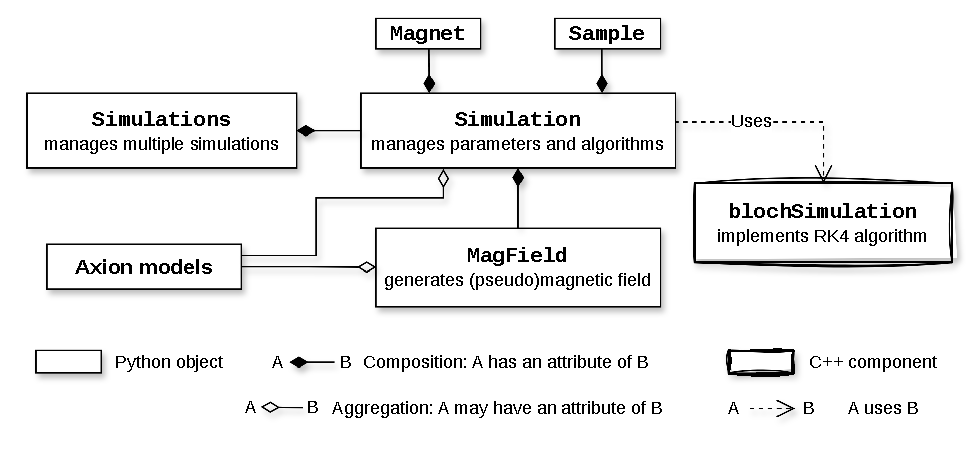
\includegraphics[width=0.8\textwidth]{figures/AxionBloch_diagram.drawio.pdf}}
    \caption{Architecture of \axionbloch{}. Each \texttt{Simulation} instance imports parameters from \texttt{Magnet}, \texttt{Sample}, and \texttt{MagField} instances. For axion simulations, axion-model objects are required both for \texttt{Simulation} to configure the simulation and for \texttt{MagField} to generate the pseudomagnetic field. \texttt{Simulations} manages one or multiple \texttt{Simulation} instances. Numerical integration is performed via the \texttt{blochSimulation} API, which provides Python access to the underlying C++ implementation. 
    }
    \label{fig:architecture}
\end{paperwidefigure}

On the Python side, classes \texttt{Sample}, \texttt{Magnet}, and \texttt{MagField} encapsulate the relevant experimental parameters, including sample relaxation times, magnetic field strength, and inhomogeneity. 
The axion models are implemented by dedicated classes, such as \texttt{MilkyWayAxionHalo}, which carry the properties of the axion fields. Together with the method \texttt{MagField.setAxionFields()}, the pseudomagnetic fields can be generated. 
Different axion models can be incorporated as separate classes without modifying the simulation framework. 
Simulation is handled within the \texttt{axionbloch.SimuTools} module. 
In particular, the classes \texttt{Simulation} and \texttt{Simulations} manage the interaction between experimental configurations and axion models, organizing the parameters and execution of single or multiple simulation runs. 

The RK4 algorithm is implemented in a dedicated C++ library. 
The application programming interface (API) for this library is \texttt{blochSimulation}. 
This C++ backend is interfaced with Python using \texttt{pybind11},\footnote{\url{http://pybind11.readthedocs.io/}} enabling cooperation between high-level Python workflow management and low-level efficient numerical computation. 


\subsection{Calibration}
\label{sec:calibration}

Accurate calibration is essential to ensure that the simulated signals reliably reflect the underlying physical system and can be compared with experimental observables. 
In particular, calibration examines the correspondence between the NMR signal and model parameters, including magnetic fields, nuclear spin gyromagnetic ratio $\gamma$, and relaxation times ($T_1$, $T_2$, and $T_2^*$). 
It allows one to verify the correctness and stability of the numerical implementation. 
In this section, examples of calibration simulations are presented along with theoretical predictions, demonstrating the methodology of calibration. 
A quantitative analysis is included at the end of the section. 
For the examples in the section, an ethanol sample and an axial bias field $\boldsymbol{B_{0}} = B_0 \boldsymbol{\hat{e}}_z$ are used. 

\subsubsection{Pulsed-NMR: free decay and spin echo}
\label{sec:pNMR}
In the pulsed-NMR calibration, one $\SI{90}{\degree}$ and one $\SI{180}{\degree}$ magnetic-field pulse are applied in the simulation. 
The magnetization is expected to\,\cite{CPMG, Abragam1961_NuclearMagnetism}:
\begin{itemize}
    \item oscillate at the Larmor frequency;
    \item be tipped by $\SI{90}{\degree}$ to the x-y plane by the $\SI{90}{\degree}$ pulse;
    \item free decay with relaxation time $T_2^*$ in the absence of pulses;
    \item refocus (echo) after $\SI{180}{\degree}$ pulses; 
    \item show decaying amplitude of echoes with relaxation time $T_2$.
\end{itemize}
The behaviors described above can be found in the calibration example illustrated in \cref{fig:calibration_T2_T2star}\,(a), indicating correct simulation behavior. 
With such a benchmark, magnetic pulses, Larmor precession, and transverse relaxations ($T_2$ and $T_2^*$) can be calibrated. 

\begin{paperwidefigure}[htb]
    \centering
    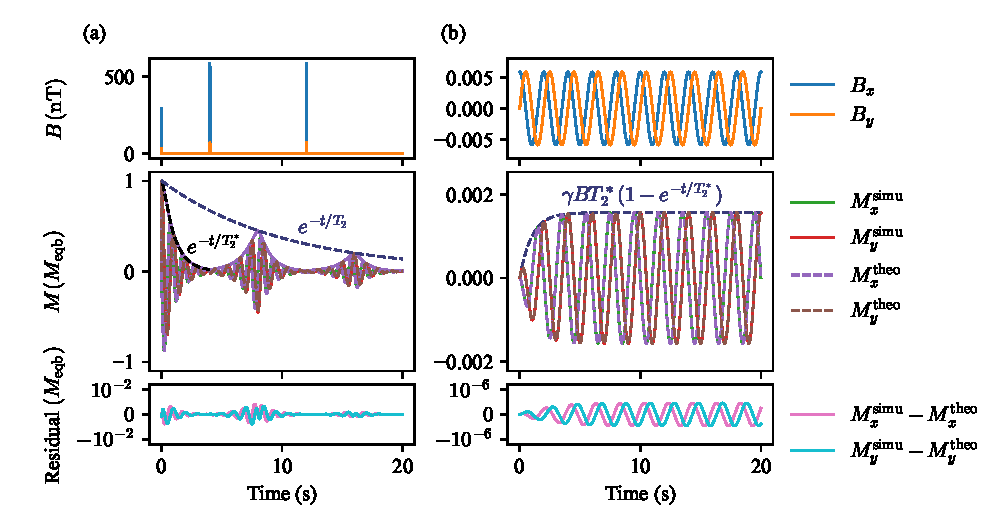
\includegraphics[width=0.9\textwidth]{figures/SpinEcho_and_CW.pdf}
    \caption{Simulated magnetic fields in x and y directions (upper row) and induced NMR signals (lower row). The magnetizations plotted are normalized by equilibrium magnetization. (a) After $\SI{90}{\degree}$ and $\SI{180}{\degree}$ magnetic-field pulses in x-y plane, free decay (relaxation time $T_2^*$) and echo signals (relaxation time $T_2$) are generated. (b) Excited by a weak CW magnetic field, the NMR signals increase with $\gamma B T_2^* (1 - e^{-t/T_2^*})$, where $B = \sqrt{B_x^2+B_y^2}$ is the magnitude of the excitation. 
    }
    \label{fig:calibration_T2_T2star}
\end{paperwidefigure}


\subsubsection{Continuous-wave NMR}
\label{sec:CW_NMR}
In the continuous-wave (CW) NMR calibration, an oscillating magnetic field is applied. 
When the magnetic field strength $B$ is weak ($\gamma B T_2^*\ll 1$) and on resonance, the transverse magnetization grows with $\gamma B T_2^* (1 - e^{-t/T_2^*})$\,\cite{Abragam1961_NuclearMagnetism}.
One such example is illustrated in \cref{fig:calibration_T2_T2star}\,(b). 
The simulation produces the expected results.
With such a benchmark, the Larmor precession and $T_2^*$ relaxation can be calibrated. 

\subsubsection{Hyperpolarized sample}
\label{sec:hyperpol}

To achieve better sensitivity to the axion field, hyperpolarization is favored in experiments. Compared to thermal polarization at room temperature, hyperpolarization techniques can boost the polarization by orders of magnitude to the order of unity. 
The \axionbloch{} package handles the polarization by the \texttt{Sample} class. 
A \SI{1}{\percent}-polarization ethanol sample is used as an example demonstrating the evolution of polarization due to the $T_1$ relaxation. 
At first ($t\ll T_1$), the polarization should exponentially decay with time constant $T_1$, until it reaches equilibrium after many $T_1$. 
As can be seen in \cref{fig:calibration_T1_HP}, the simulated $T_1$ relaxation agrees with the expected behavior. 
More of such simulations can be applied in calibrating $T_1$ relaxation. 

\begin{figure}
    \centering
    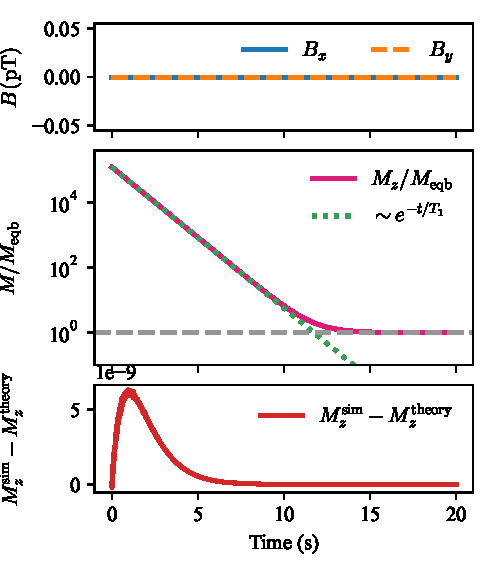
\includegraphics[width=0.45\textwidth]{figures/T1_hyperpolarized.pdf}
    \caption{
    Simulated $T_1$ relaxation of a hyperpolarized sample in a static bias field. The axial magnetization $M_z$ is normalized by the equilibrium magnetization $M_\mathrm{eqb}$. 
    }
    \label{fig:calibration_T1_HP}
\end{figure}


\subsubsection{Quantitative evaluation}

The accuracy of simulations is evaluated by the discrepancy between the theoretically expected magnetization and simulation results, characterized by
\begin{equation}
    \chi^2 = \dfrac{\sum |M_\mathrm{expected} - M_\mathrm{simu}|^2}{\sum |M_\mathrm{simu}|^2}
    \,. 
    \label{eq:chisq}
\end{equation} 
Here $M_\mathrm{expected}$ and $M_\mathrm{simu}$ are magnetization expected and simulated, respectively. 
$\sum$ denotes the sum over integration steps.
A well-calibrated simulation should give $\chi^2\ll 1$. 
Calibration scripts are stored in the test suite of \axionbloch{}. 
In each calibration, parameters such as Larmor frequency and relaxation times are varied over orders of magnitude to cover all possible cases in simulation.
The results of the calibrations are summarized in \cref{tab:calibration_summary}. 
The discrepancies are generally small ($\chi^2 < 10^{-4}$).
If a certain simulation precision is required, the $\chi^2$ value serves as a quantitative reference. 

% \begin{table}[H] 
% %\small % Change table font size
% \caption{This is a table caption. Tables should be placed in the main text near the first time they are~cited.\label{tab1}}
% %\isPreprints{\centering}{} % Only used for preprints
% \begin{tabularx}{\textwidth}{CCC}
% \toprule
% \textbf{Title 1}	& \textbf{Title 2}	& \textbf{Title 3}\\
% \midrule
% Entry 1		& Data			& Data\\
% Entry 2		& Data			& Data \textsuperscript{1}\\
% \bottomrule
% \end{tabularx}

% \noindent{\footnotesize{\textsuperscript{1} Tables may have a footer.}}
% \end{table}

\begin{paperwidetable}
\small % Change table font size
\caption{Summary of calibrations. $\chi^2$ indicating the discrepancy is defined in \cref{eq:chisq}; $\chi^2\ll 1$ indicates a well-calibrated simulation. Here $\nu_\mathrm{L}$ stands for Larmor frequency, determined by the bias magnetic field. $\nu_\mathrm{RCF}$ is RCF frequency. $\nu_\mathrm{L}$ and $\nu_\mathrm{RCF}$ are varied from \SI{1}{\kHz} to \SI{1}{\GHz}. The bias field inhomogeneity is swept from \SI{.1}{\ppm} to \SI{20}{\ppm}. $T_1$ ranges from \SI{1}{\ms} to \SI{1}{\kilo\second}. The integration step size is chosen to be $T_2^* / 500$. Finer step sizes yield lower $\chi^2$ at increased computational cost. More technical details of the calibrations can be found in the test suite.\label{tab:calibration_summary}}
\resizebox{\linewidth}{!}{%
\begin{tabular}{lllll}
    \toprule
    \textbf{Calibration} &
    \textbf{Parameters calibrated} &
    \textbf{Varied parameters} &
    $\bm{\chi^2}$ &
    \textbf{Dominant source of error} \\
    \midrule
    Pulsed NMR: free decay &
    Pulse amplitude, $\nu_\mathrm{L}$, $T_2^*$, $T_2$ &
    $\nu_\mathrm{RCF}$ &
    $<10^{-4}$ &
    Finite number of steps for hard pulses. \\
    CW-NMR &
    $\nu_\mathrm{L}$ and $T_2^*$ &
    $\nu_\mathrm{RCF}$ &
    $<10^{-5}$ &
    Finite integration step size. \\
    $T_1$ relaxation &
    $T_1$ &
    $\nu_\mathrm{RCF}$, $\nu_\mathrm{L}$, initial polarization &
    $<10^{-7}$ &
    Finite integration step size. \\
    \bottomrule
\end{tabular}
}%
\end{paperwidetable}


\subsection{Axion simulation}
\label{sec:simulation}

Similar to the calibration examples, axion-induced NMR signals are generated by solving the Bloch equations with the axion-induced pseudomagnetic field as part of the effective magnetic field. 
An example of a commonly considered model -- axion constituting the Milky Way galactic dark matter halo\,\cite{Evans2019_SHMRefined,Gramolin2022Feb_SpectralSignatures} is implemented in the class \texttt{MilkyWayAxionHalo}. 
In this model, the axion field is treated as an oscillating field with a frequency determined by the axion mass, and a linewidth (characterizing the stochasticity) determined by the velocity dispersion of the virialized dark matter halo. 
The sample is chosen to be \ch{^{129}Xe}, polarized to $\SI{50}{\percent}$ initially, and the bias field is applied along the z direction. 
The details of the simulation configuration can be found in the code example in \cref{code:axion_example}. 
Readers are referred to \cref{fig:architecture} which illustrates the relationship between the objects in the code example. 
The simulated pseudomagnetic fields and the amplitude of the induced transverse magnetization are shown in \cref{fig:MilkyWayAxionHalo}, in which the signal increases with time at the beginning of the simulation due to the pseudomagnetic field, and then decays due to the $T_1$ relaxation. 
The efficiency of the simulation is limited by time consumption for the numerical integration of the Bloch equations. 
The total number of integration steps $N$ can be found by
\begin{align}
    N &= \text{\texttt{Simulation.rate}} \times \text{\texttt{Simulation.duration}} \nonumber\\
    &\quad \times \text{\texttt{MagField.numFields}} \times \text{\texttt{Magnet.numPt}}\,,
\end{align}
where \texttt{Simulation.rate} and \texttt{Simulation.duration} are the simulation rate and duration, \texttt{MagField.numFields} is the number of random pseudomagnetic fields generated to account for the stochasticity of the axion field, and \texttt{Magnet.numPt} is the number of bias fields sampled to account for the inhomogeneity of the bias field. 

To accelerate the simulation, the independent realizations of the (pseudo)magnetic fields are parallelized using Open Multi-Processing (OpenMP)\,\cite{OpenMP2024} in \texttt{blochSimulation}.
The number of OpenMP threads is controlled by the runtime environment and may therefore vary with the user's hardware and OpenMP settings.
The spin-packet and time-stepping loops within each realization were evaluated serially. 

For the example in \cref{code:axion_example}, the total number of integration steps is \SI{7e8}{}, and the runtime is \SI{2.7}{\s} on a personal computer (CPU: Intel\textsuperscript{\textregistered} Core\textsuperscript{\texttrademark} Ultra 7 155H; base speed: 1.40\,GHz). 
Such moderate runtime allows users to explore different parameter regimes with many simulations. 

\begin{figure}
\center
\fbox{%
  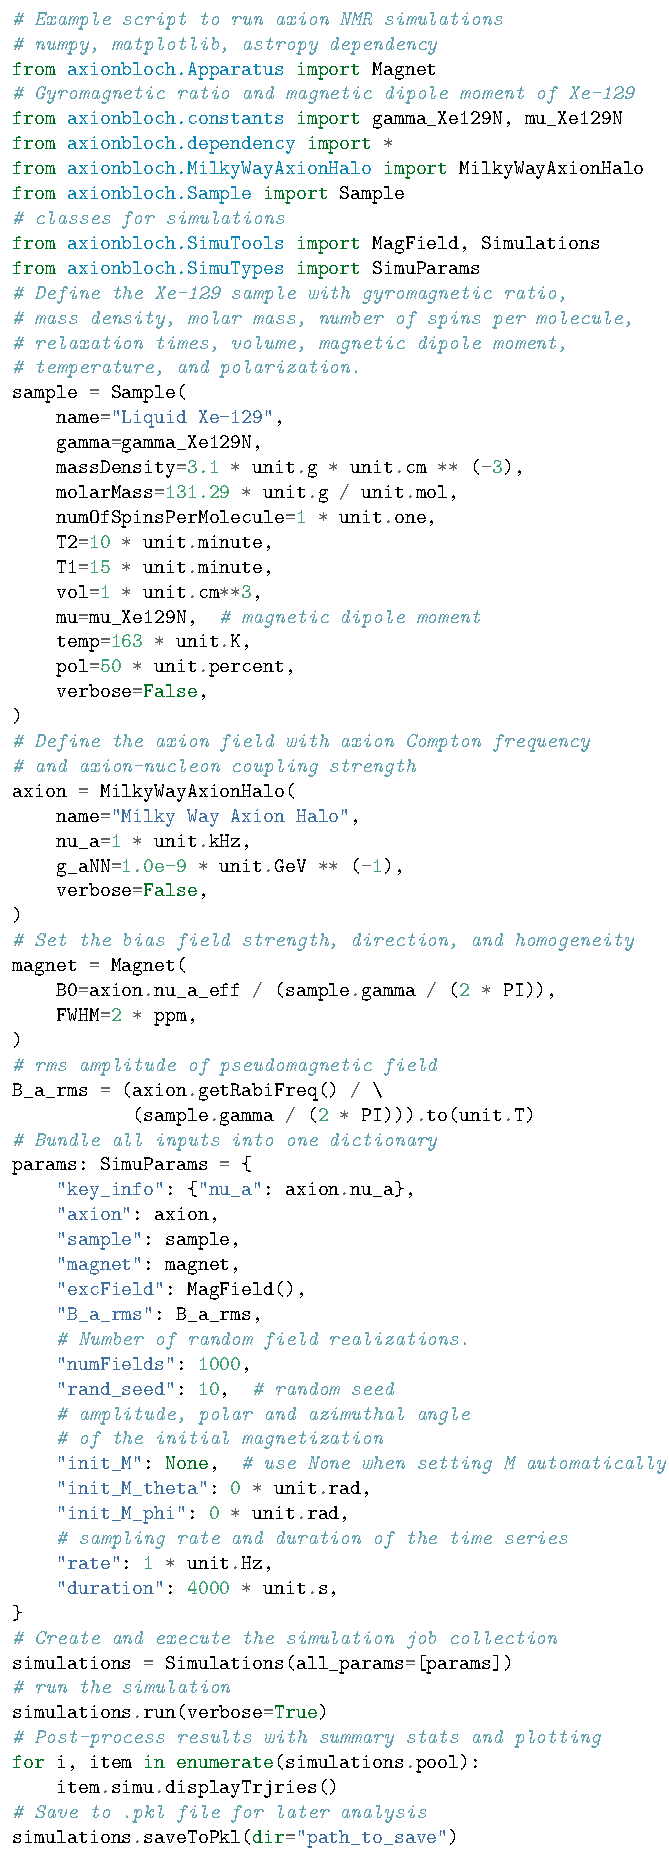
\includegraphics[
    % width=0.9\linewidth,
    height=0.9\textheight,
    keepaspectratio,
    clip
  ]{figures/axion_example.pdf}%
}% \vspace{0.1in}
\caption{Example code of an axion simulation.}
\label{code:axion_example}
\end{figure}

\begin{paperwidefigure}[htb]
    \centering
    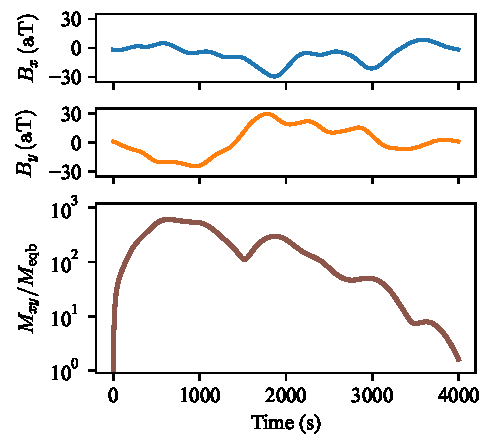
\includegraphics[width=0.45\textwidth]{figures/MilkyWayAxionHalo-1.pdf}
    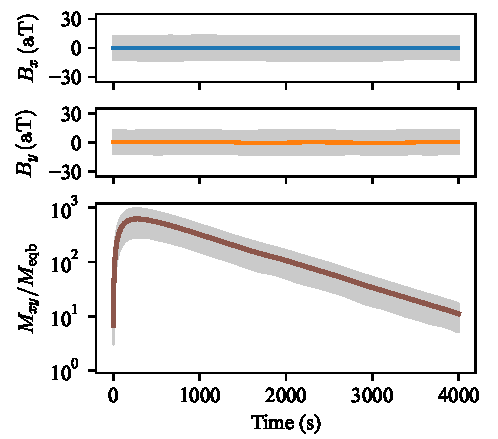
\includegraphics[width=0.45\textwidth]{figures/MilkyWayAxionHalo-1000.pdf}
    \caption{Simulations of local virialized axion dark matter halo. From top to bottom: pseudomagnetic fields in the transverse plane ($B_x$ and $B_y$) and the transverse magnetization normalized by the equilibrium magnetization ($M_{xy}/M_\mathrm{eqb}$). Left: one single simulation. Right: 1000 simulations to account for the stochasticity. The solid lines indicate the value (left column) or mean value (right column) of $B_x$, $B_y$, and $M_{xy}$, while the gray shadows indicate the $\pm \sigma$ (standard deviation) range. The sample for the simulations is assumed to be polarized to $\SI{50}{\percent}$ initially.
    }
    \label{fig:MilkyWayAxionHalo}
\end{paperwidefigure}


\section{Development}
\label{sec:dev-approach}


% Version Control
Development of \axionbloch{} is managed using \texttt{git},\footnote{\url{http://git-scm.com}} with the code hosted on a public GitHub repository.\footnote{\url{https://github.com/Yuzhe98/AxionBloch}} 
Changes to the main codebase follow a \textit{pull request} workflow, allowing contributions to be reviewed before being merged. Users can participate by forking the repository, making modifications in their fork, and submitting pull requests for review by the developers.
As \axionbloch{} is intended as a collaborative resource, user contributions and suggestions are encouraged and appreciated. 

% Automated Testing with pytest
\axionbloch{} includes a suite of automated tests to ensure correctness and reliability. 
The tests are implemented using the \texttt{pytest} framework,\footnote{\url{https://docs.pytest.org/}} which allows for calibration of physical processes and testing of functions, classes, and modules. 
The test suite covers core functionalities such as:
\begin{itemize}
    \item initialization and manipulation of classes; 
    \item numerical integration of the Bloch equations;
    \item magnetic fields and relaxations;
    \item handling of each axion field configuration.
\end{itemize}
Tests can be executed locally. In the future, tools may be added for online testing considering the demand of testing. 

% documentation
Documentation for \axionbloch{} is available on Read the Docs.\footnote{\url{http://axionbloch.readthedocs.io}}
It is built using \texttt{Sphinx}\footnote{\url{http://www.sphinx-doc.org}} and provides detailed explanations of the API, along with instructions for installation, configuration, and usage.

% Future
As numerous new axion models and experiments are emerging, the functionality of \axionbloch{} may extend so that it can be a tool for updating our knowledge of the induced spin dynamics. 
Furthermore, capabilities for simulating zero-to-ultra-low-field (ZULF) NMR will be implemented in future versions. 


\section{Conclusions}
\label{sec:conclusions}


\axionbloch{} has been presented as a framework for simulating spin dynamics induced by magnetic fields or axion fields under a variety of physical scenarios. 
The package adopts SI units so that the inputs and outputs are directly comparable to experimental parameters and observables. 
Numerical integration of the Bloch equations is performed using a fourth-order Runge--Kutta method in the rotating coordinate frame, enabling stable and efficient simulation. 
Comprehensive calibrations have been performed to ensure the accuracy of the simulations.
An example simulation of axion-induced signals from a local virialized axion dark matter halo is presented to demonstrate the package's capabilities. 

By providing an open-source, well-documented, and tested tool, \axionbloch{} aims to facilitate the study of axion-induced spin dynamics in precision measurement experiments and to serve as a platform for further method development and incorporation of new axion models.

Note that this package can be of interest to the NMR community for its applications in, for example, educational purposes. 
For example, students can specify pulse sequences for the simulation and see the visualized simulation results. 



% \authorcontributions{Conceptualization, methodology, software, validation, formal analysis, investigation, and writing---original draft preparation, Yuzhe Zhang; writing---review and editing, Yuzhe Zhang.}

\funding{This work has been supported by the Cluster of Excellence ``Precision Physics, Fundamental Interactions, and Structure of Matter'' (PRISMA++ EXC 2118/2) funded by the
German Research Foundation (DFG) within the German Excellence Strategy (Project ID 390831469).}

\institutionalreview{Not applicable.}

\informedconsent{Not applicable.}

\dataavailability{The data and code that generate this manuscript are available at \url{https://github.com/Yuzhe98/AxionBloch-paper}.}

\acknowledgments{The author acknowledges helpful discussions with Hendrik Bekker, Dmitry Budker, and Alexander Sushkov, and thanks the CASPEr Collaboration for its support. 
The author is grateful to the communities supporting the open-source software and tools: \texttt{git}, \texttt{NumPy}, 
\texttt{SciPy}\footnote{\url{https://docs.scipy.org/}}\,\cite{Virtanen2020_SciPy}, 
\texttt{matplotlib}\footnote{\url{https://matplotlib.org/}}, 
\texttt{astropy}, 
\texttt{pybind11}, 
\texttt{IPython}\footnote{\url{https://ipython.org/}}\,\cite{Perez2007_IPython}, 
\texttt{Jupyter}\footnote{\url{https://jupyter.org/}}\,\cite{Granger2021_Jupyter}, 
\texttt{pytest}, 
\texttt{Sphinx}, 
GitHub\footnote{\url{https://github.com/}} 
and 
Read the Docs\footnote{\url{https://about.readthedocs.com/}}. }

\conflictsofinterest{The author declares no conflicts of interest.}

\reftitle{References}
\bibliography{references}
\PublishersNote{}
\end{document}
